\documentclass[conference]{IEEEtran}
\IEEEoverridecommandlockouts
% The preceding line is only needed to identify funding in the first footnote. If that is unneeded, please comment it out.
\usepackage{cite}
\usepackage{amsmath,amssymb,amsfonts}
\usepackage{algorithmic}
\usepackage{graphicx}
\usepackage{textcomp}
\usepackage[utf8]{inputenc}
\usepackage[english]{babel}
\def\BibTeX{{\rm B\kern-.05em{\sc i\kern-.025em b}\kern-.08em
    T\kern-.1667em\lower.7ex\hbox{E}\kern-.125emX}}
\begin{document}

\title{Dispozitiv de monitorizare a somnului\\
{\footnotesize \textsuperscript{}}
\thanks{}
}

\author{\IEEEauthorblockN{Ignatescu Nicolas}
\IEEEauthorblockA{\textit{Universitatea Politehnica București} \\
\textit{Facultatea de Inginerie Medicală}\\
București România \\
nicolas.ignatescu@gmail.com}
\and
\IEEEauthorblockN{Munteanu Cristian}
\IEEEauthorblockA{\textit{Universitatea Politehnica București} \\
	\textit{Facultatea de Inginerie Medicală}\\
	București România \\
	cristi.munteanu19@yahoo.ro}

}

\maketitle

\begin{abstract}
Somnul este o parte necesara si obligatorie a fiecarei zile din viata noastra, insa exista diferite afectiuni ce pot afecta calitatea acestuia, odihna propriu-zisa, din timpul noptii si pot avea consecinte asupra vietii individului. Un indiciu al calitatii somnului este activitatea motorie sau miscarile pe care le facem in timpul somnului. Un studiu publicat in 2014, face o serie de observatii care arata corelatia dintre afectiuni psihologice si lipsa somnului, cu cresterea miscarilor in timpul somnului, studiu realizat in perioada de copilarie si adolescent ale subiectilor \cite{childsleep}. Astfel, dispozitivul de monitorizare a somnului  masoara si identifica aceasta activitate din timpul somnului. Dispozitivul se bazeaza pe o retea de senzori piezoelectrici care sunt montati in saltea. 
\end{abstract}

\begin{IEEEkeywords}
component, formatting, style, styling, insert
\end{IEEEkeywords}

\section{Introduction}
This document is a model and instructions for \LaTeX.
Please observe the conference page limits. 

\section{Ease of Use}

\begin{table}[htbp]
\caption{Table Type Styles}
\begin{center}
\begin{tabular}{|c|c|c|c|}
\hline
\textbf{Table}&\multicolumn{3}{|c|}{\textbf{Table Column Head}} \\
\cline{2-4} 
\textbf{Head} & \textbf{\textit{Table column subhead}}& \textbf{\textit{Subhead}}& \textbf{\textit{Subhead}} \\
\hline
copy& More table copy$^{\mathrm{a}}$& &  \\
\hline
\multicolumn{4}{l}{$^{\mathrm{a}}$Sample of a Table footnote.}
\end{tabular}
\label{tab1}
\end{center}
\end{table}

\begin{figure}[htbp]
\centerline{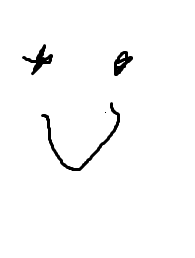
\includegraphics{fig1.png}}
\caption{Example of a figure caption.}
\label{fig}
\end{figure}



\section*{Acknowledgment}







\bibliographystyle{IEEEtran}
\bibliography{bibliografie}

\end{document}
